\message{ !name(test.tex)}\documentclass{beamer}
\usetheme{Madrid}
\usepackage{palatino}
\usepackage{tikz}
\usepackage{graphicx}

% Définition de l'environnement pour la figure d'Awalé avec un nombre variable de paramètres pour les pierres

\date[]{}
\title[La recherche du meilleur coup.]{À la recherche du meilleur coup au jeu d'Awalé}
\author[Nils Lelorieux]{Nils Lelorieux}
\institute[]{numéro de candidat : 24296}

\begin{document}

\message{ !name(test.tex) !offset(-3) }


\begin{frame}
  \titlepage
\end{frame}
 
\begin{frame}
  \frametitle{Introduction}


  \begin{minipage}[b]{0.3\linewidth}
    \begin{figure}
      \centering
      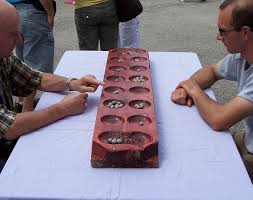
\includegraphics[width=1.5\linewidth]{ressources/photo_joueur_awale.jpeg}
      \caption{Une partie d'Awalé}
      \label{fig:mon_image}
      %% \label{fig:1}
    \end{figure}
  \end{minipage}
  \hfill
  \begin{minipage}[b]{0.48\linewidth}
    \begin{figure}
      \centering
      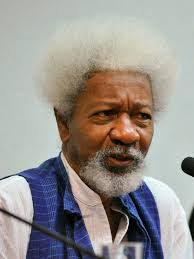
\includegraphics[width=0.8\linewidth]{ressources/wole_soyinka.jpeg}
      \label{fig1}
      \caption{Photographie de Wole Soyinka}
    \end{figure}
  \end{minipage}
      
\end{frame}

\begin{frame}
  \frametitle{Un jeu ancien et important}
  \begin{figure}
    \centering
    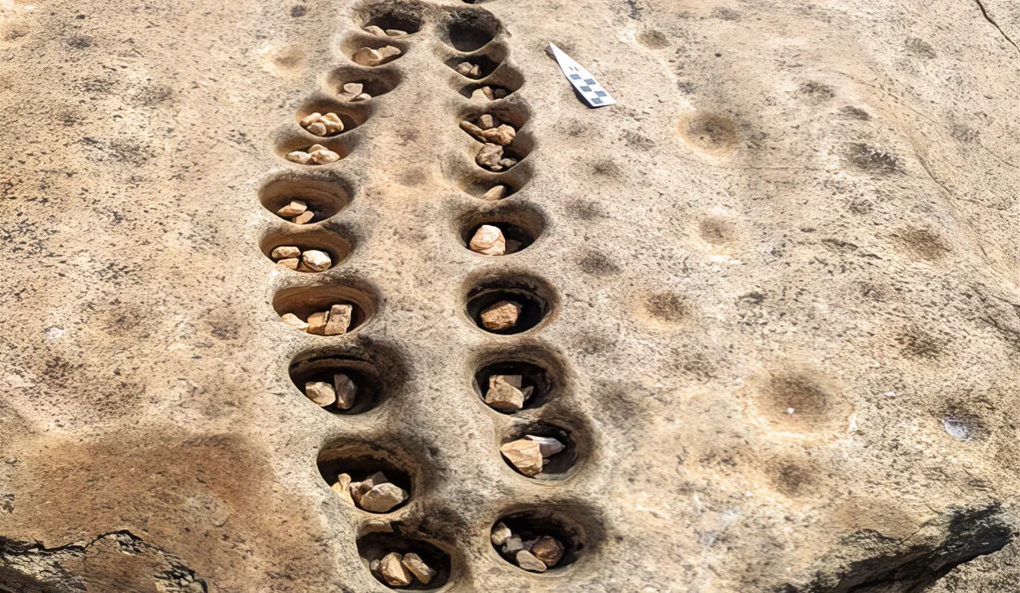
\includegraphics[width=\linewidth]{ressources/ancien_plateau_jeu.png}
    \caption{Un ancien plateau de jeu decouvert au Kenya}
  \end{figure}
\end{frame}


\begin{frame}
  \frametitle{Vue d'ensemble}
  \tableofcontents
\end{frame}


\section{Présentation des règles du jeu et motivations}
\begin{frame}
  \frametitle{Règles du jeu}
  \begin{minipage}[t]{0.5\linewidth}
    \begin{itemize}
    \item<Règles du jeu>
    \item Deux joueurs s'affrontent.
    \item 4 graines dans les 12 trous divisé en 2 rangée de 6.
    \item Le premier joueur choisi un puit et sème les graines.
    \item Si le dernier puit semé a 2 ou 3 pierres, il les récupère et fait la même chose dans le puit précédent, ...
      \item Le gagnant est le joueur qui a le plus de pierres
    \end{itemize}
  \end{minipage}
  \hfill 
  \begin{minipage}[t]{0.49\linewidth}
    \begin{figure}
      \centering
      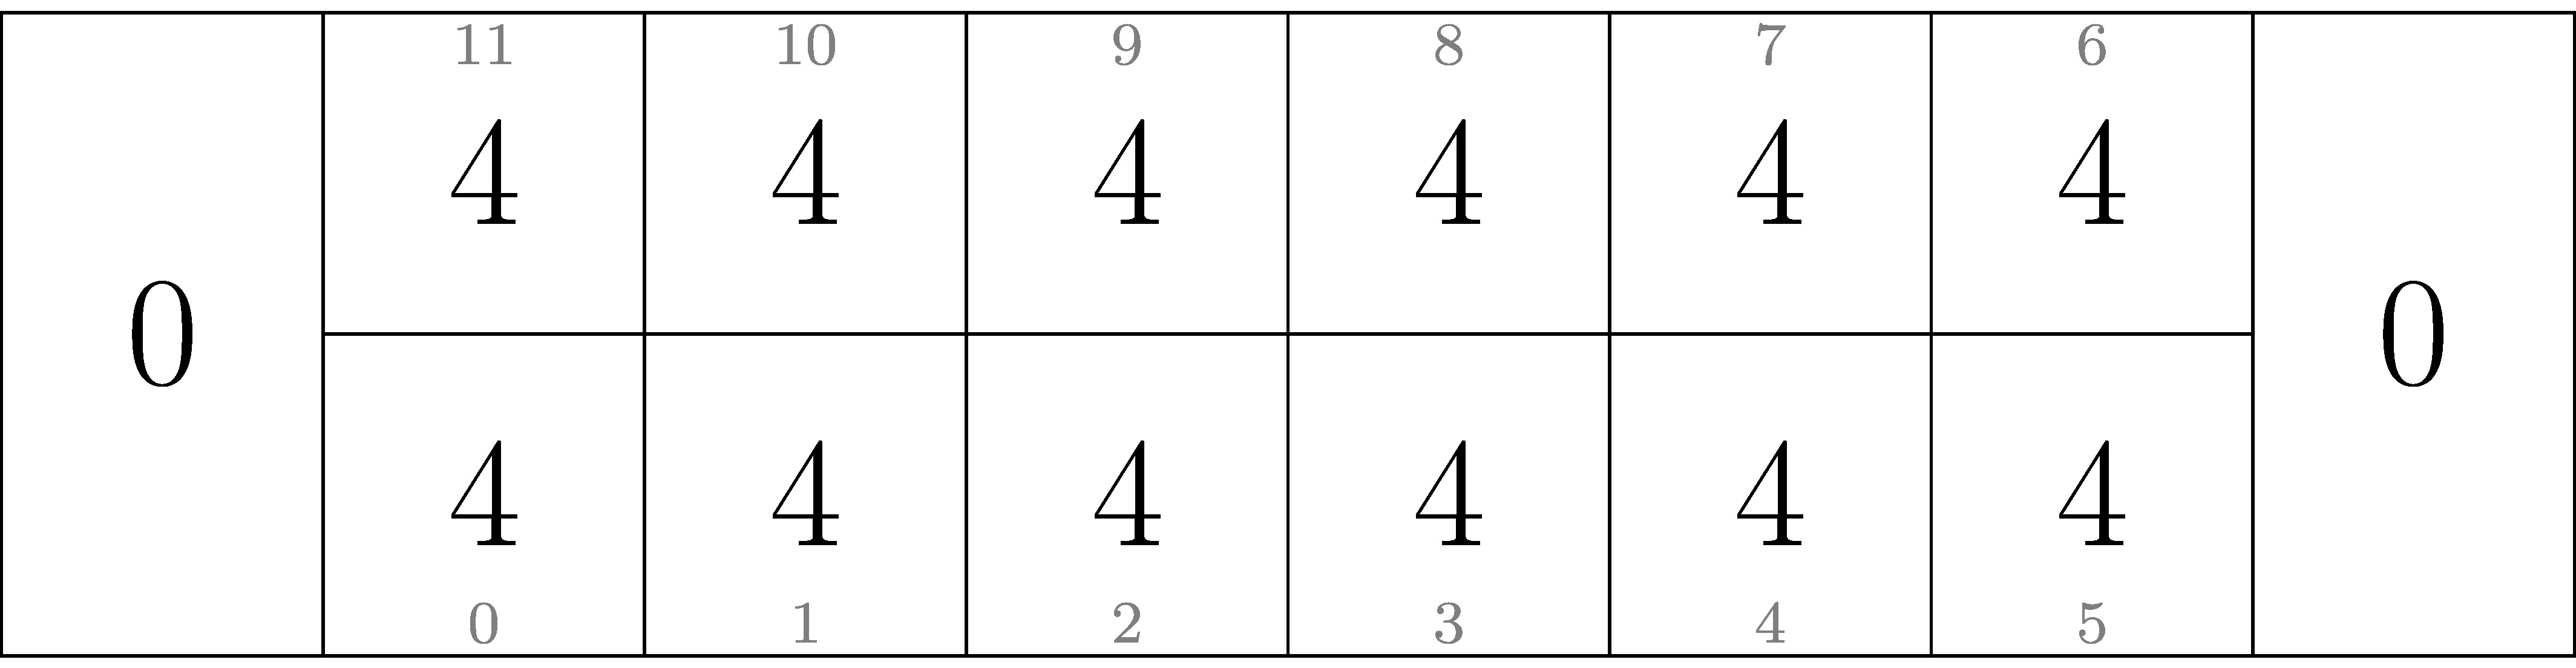
\includegraphics[width=1.05\linewidth]{ressources/p_debut.pdf}
      \caption{L'état du plateau au début de la partie}
    \end{figure}
    
  \end{minipage}
  
\end{frame}

\section{Échec de l'approche théorique et des premiers algorithmes}
\begin{frame}
  \frametitle{Une approche théorique}
  
\end{frame}

\section{Des résultats concluents grâce à deux nouvelles techniques : la recherche arborescente de Monte-Carlo et l'analyse rétrograde}
\begin{frame}
  \frametitle{Un problème bien connu}
  
\end{frame}




\end{document}

%%% Local Variables:
%%% mode: LaTeX
%%% TeX-master: t
%%% End:

\message{ !name(test.tex) !offset(-111) }
